\subsection{Integration Testing Plan Definition}

\subsubsection{Microservices}

\descriptionproblem
Consider the microservice-based architecture shown in Figure~\ref{fig: microservice-based architecture}. The architecture is organized into eight stateless microservices collaborating to fulfill requests $R1$ and $R2$. $S1$ is the front-end service that receives both requests. The fulfillment of request $R1$ requires the interaction with services $S2$ and $S3$ (through sub-requests $R1.1$ and $R1.2$, respectively), which, in turn, need to interact with other services. In particular, $S2$ interacts with $S4$ and $S5$ and $S3$ with $S5$ and $S6$. The fulfillment of $R2$ requires that $S1$ interacts with $S8$, which, in turn, interacts with $S6$ and $S7$.

\begin{figure}[!htp]
    \centering
    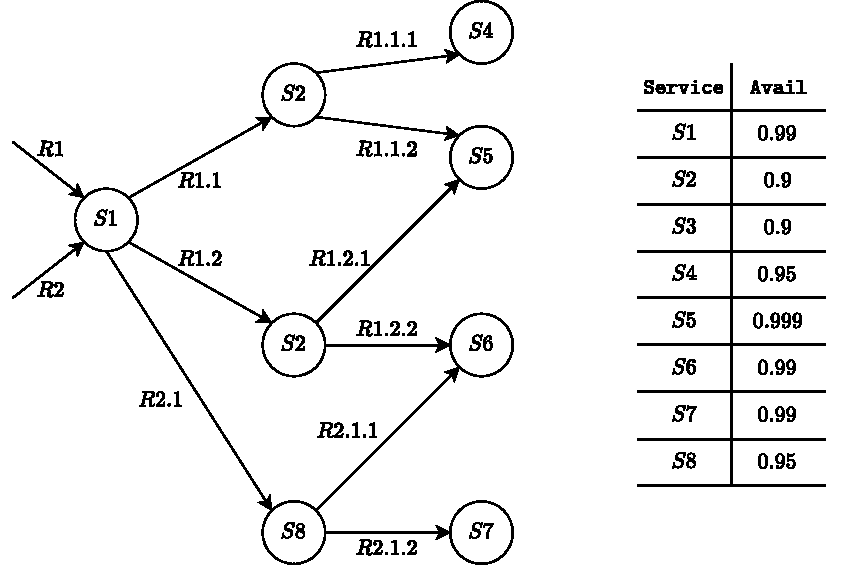
\includegraphics[width=\textwidth]{img/microservices-1.pdf}
    \caption{Microservice-based architecture.}
    \label{fig: microservice-based architecture}
\end{figure}

\questionproblem
\begin{enumerate}
    \item Define an integration and test plan for the architecture, motivating your choice.

    \item Assume that we are asked to test whether the availability improvement theoretically obtained with the duplication of services is actually achieved. How would we proceed to perform such a test?
\end{enumerate}

\solution
\textbf{\underline{Solution 1}.} The strategy used for integration testing (a summary of the strategies can be found in Figure~\ref{fig: summary of integration test strategies} on page~\pageref{fig: summary of integration test strategies}) is the iterative/incremental strategy.

In particular, we use the \emph{Threads} strategy to test some of the modules. This is possible because the set of modules together provide a user-visible programme function.

We also use a \emph{hierarchical} strategy with a \emph{top-down} approach because the modules are integrated and all functionality can be tested.

The test plan can be divided into $R1$ and $R2$ for the given architecture. Given the request $R1$, we can test a part of the architecture. Meanwhile, given the request $R2$, we can test the remaining part of the architecture. Then, the test plan is the following:
\begin{enumerate}
    \item Integration of the $S1$ (front-end) and testing by emulating two requests called $R1$ and $R2$. We need the following stubs to test this service: $R1.1$, $R1.2$ and $R2.1$.

    \item Once completed, we temporarily leave aside $R2$ and implement the $R1$ tree. We start from the $S2$ and $S3$ by creating the requests $R1.1.1$, $R1.1.2$, $R1.2.1$ and $R1.2.2$ as stubs. Now we can also test the triangles $S1$, $S2$ and $S3$.

    \item Finally, we implement $S4$, $S5$ and $S6$. We do not use stubs to test these services because the other modules have already been implemented ($S2$, $S3$). At this point, the request $R1$ has been thoroughly tested and integrated.

    \item We can now integrate the $R2$ tree. We implement/test the service S8 by using $R2.1.2$ as stubs. The $S6$ was already implemented (previous step), so we can use that module directly.
    
    \item Finally, we implement $S7$ and test the whole architecture because all the services are implemented.
\end{enumerate}

\highspace
\textbf{\underline{Solution 2}.} To measure the quantitative impact of architectural decisions, we use the availability metric (Formula~\ref{eq: availability metric} on page~\pageref{eq: availability metric}).

\highspace
The main values required are MTTR (Mean Time To Repair) and MTTF (Mean Time To Failures). If we want to do some tests to compare the two architectures before and after duplication, we can run the application for a long time and simulate a failure of one of the services. We can then calculate the time taken by the architecture to restore the service. The requests can be made sequentially or in parallel to study how the architecture responds.

\highspace
Using the availability metric, we can understand if the chosen replication makes sense and if the availability is better than the architecture without duplication of services.